\section{Conclusões}

A prática permitiu compreender o circuito gerador de onda triangular, uma categoria de circuitos geradores utilizando amplificadores operacionais, de modo a gerar uma onda triangular a partir de um circuito comparador não-inversor com histerese em cascata com um circuito integrador.

Podemos notar que os resultados obtidos na prática, no geral, estão de acordo com o que foi previsto na análise teórica, além de possibilitar a geração de uma onda quadrada na saída do comparador. Portanto, mesmo com as dificuldades impostas na análise teórica, a prática  permitiu-nos relacionar os conceitos aprendidos em sala com que realmente acontece em laboratório.

%\newpage

\section{Anexos}

\begin{figure}[H] 
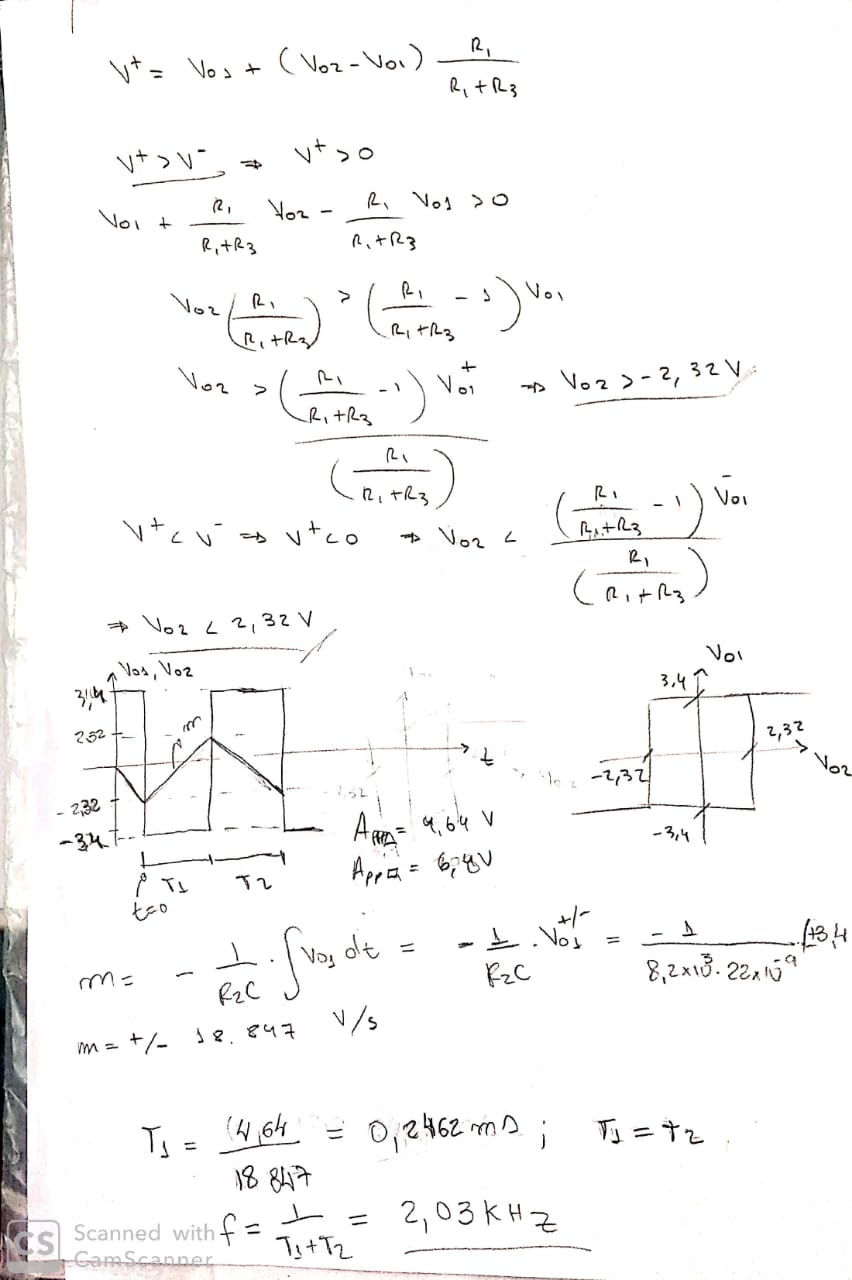
\includegraphics[scale=0.4]{images/calc.jpeg} 
\centering
\caption{Folha de cálculos da prática.}
\label{p5-2} 
\end{figure} 
